\documentclass[conference]{IEEEtran}
\IEEEoverridecommandlockouts
% The preceding line is only needed to identify funding in the first footnote. If that is unneeded, please comment it out.
%Template version as of 6/27/2024

\usepackage{cite}
\usepackage{amsmath,amssymb,amsfonts}
\usepackage{algorithmic}
\usepackage{graphicx}
\usepackage{textcomp}
\usepackage{caption}
\usepackage{xcolor}
\usepackage{float}
\usepackage{url}


\def\BibTeX{{\rm B\kern-.05em{\sc i\kern-.025em b}\kern-.08em
    T\kern-.1667em\lower.7ex\hbox{E}\kern-.125emX}}
\begin{document}

\title{Tumor Detection and Explainability using Gradient-weighted Class Activation Mapping}

\author{\IEEEauthorblockN{Brendan George Lauterborn}
\IEEEauthorblockA{\textit{Department of Computer Science} \\
\textit{Towson University}\\
Towson, United States \\
blaute3@students.towson.edu}
}


\maketitle
\begin{abstract}
Brain Tumors are often discovered among a patient in the later stages, making the chances of curing the patient dramatically lower. It can be difficult to detect tumors early because the symptoms vary depending on the person. The brain tumor can affect a person's speech, balance, behavior, and vision. The location of the tumor, the type of tumor, and its development within the brain play a large role in determining these effects. This project focuses on building a machine learning model that detects and classifies brain tumors based on Magnetic Resonance Imaging (MRI) scans using deep learning techniques. We deployed a Convolutional Neural Network (CNN) with transfer learning based on the DenseNet-121 architecture to classify MRI images into four categories. These categories are glioma, meningioma, pituitary, and healthy brain scans. To further enhance interpretability, Explainable Artificial Intelligence (XAI) methods such as Gradient-weighted Class Activation Mapping (Grad-CAM) is used to highlight the important regions of the MRI scan that influenced the model's prediction. The goal of this project is to develop a reliable medical image classification model that demonstrates the capabilities of deep learning and supports the medical field in the early detection of brain tumors.
\end{abstract}

\section{Introduction}
Brain tumors are one of the most dangerous neurological conditions that remains a problem to date. These tumors are very complex because they can grow silently and the symptoms may be mistaken for other issues. Early detection of brain tumors is critical. If a tumor is caught in the early stages, the chances of that tumor being removed safely improves to about 90\% \cite{ncneurospine}. MRIs are commonly used to look for tumors because these scans provide detailed images of the brain for the medical professionals to examine. Analyzing these MRI scans are time consuming, difficult, and take resources.

Advancements in deep learning models, CNNs specifically, have supported the growth in medical image analysis. CNNs provide a more scalable approach to image classification and analysis, especially in the medical field. This deep learning model can learn features and extract key information from images alone. More specifically, we can utilize the transfer learning technique by using a pre-trained CNN and fine-tuning this model for our specific task at hand. Transfer learning allows us to utilize a CNN model that has already been trained on a large-scale dataset so that we do not have to train from scratch. This allows for quicker and more efficient training, which results in a more accurate model for classifying tumors. In our experiment, we utilize the pre-trained model known as DenseNet-121. DenseNet-121 has proven to be strong in image classification because it mitigates the problem of vanishing gradient, improves feature reuse, and decreases parameter usage \cite{bhandari}.

Although there has been success in medical image classification, we seek to build upon this and provide more reasoning behind the decision of the model to support model predictions. More specifically, we utilize Explainable AI techniques such as Grad-CAM to achieve this task. Understanding why the model has made a certain prediction is just as important as building a model that can make a prediction. Grad-CAM helps identify the important regions of an MRI scan that contributed to the model’s decision. This improves overall reliability and supports medical professionals in their decisions.

The overall goal of this work is to demonstrate the effectiveness of deep learning and XAI techniques in supporting accurate and interpretable brain tumor detection.

\section{Dataset Description}
For this study, we used the \textit{Brain Tumor MRI Scans} dataset obtained from Kaggle. The dataset contains MRI images categorized into four classes: \textit{glioma}, \textit{meningioma}, \textit{pituitary}, and \textit{healthy}. Each image represents an MRI scan of the human brain. The dataset is organized into separate folders for each classification category, serving as the associated label that tells the tumor class. There are 1621 total glioma images, 1645 total meningioma images, 1757 total pituitary images, and 2000 total healthy images. The dataset provides a relatively balanced and diverse set of MRI scans that enables effective training and evaluation of deep learning models for brain tumor classification.

\section{Related Works}
Previous work has demonstrated the effectiveness of deep learning techniques for brain tumor detection and classification using MRI scans. Bhanothu et al. proposed a Faster R-CNN based framework using the VGG-16 architecture to detect and classify glioma, meningioma, and pituitary tumors from MRI images. Their approach led to training accuracy of 98.4\% after 120 epochs. Their model achieved average precision scores of 75.18\% for glioma, 89.45\% for meningioma, and 68.18\% for pituitary tumors. Their work also utilized Intersection over Union (IoU). From this, they are able to evaluate how accurately the predicted tumor boxes overlapped with the true tumor boxes. This work highlights the effectiveness of deep learning techniques and the ability to classify brain tumors and localize tumors based on MRI scans. \cite{bhanothu2020}

Gayanga et al. developed a CNN-based framework for detecting and analyzing brain tumor edge intensity using MRI scans. Their work focused on edge detection techniques. Some of the techniques include grayscale conversion, median filtering, CLAHE enhancement, watershed segmentation, fuzzy c-means clustering, and Canny edge detection. Their work demonstrated the importance of tumor detection and edge detection for distinguishing a malignant tumor from a benign tumor. This supports the research around deep learning models in detecting brain tumors. \cite{gayanga2019}


\section{Methodology}

\subsection{Experimental Setup}
The experimental setup was implemented in Python using the PyTorch deep learning framework and the torchvision library. All model training and testing was conducted using Google Colab with access to an NVIDIA T4 GPU. When available, CUDA acceleration was utilized to improve training and inference efficiency. The dataset was divided into training, validation, and testing sets using a 70/15/15 split, where 70\% of the data was used for training, 15\% for validation, and 15\% for testing. The batch size was set to 32 for training, validation, and testing.

\subsection{Pre-processing}

Since the dataset consists of medical imaging data, pre-processing and data augmentation techniques were applied to improve model generalization and reduce overfitting. For the training dataset, we applied random rotations up to 30 degrees, random resized cropping to 224$\times$224, and random horizontal flipping were applied. These augmentations are applied to increase variability. The model is able to learn more robust features from the images when these augmentations are applied to them.

For the validation and testing splits, we resized the images to 255$\times$255 before cropping. From there, we center crop the images to the size 224$\times$224. Unlike the training split where we add randomness to the images, in the validation and testing splits we want to ensure consistent evaluation across all images.

All images were converted to tensors and normalized using the ImageNet mean and standard deviation values: mean = [0.485, 0.456, 0.406] and standard deviation = [0.229, 0.224, 0.225]. These normalization values were used because transfer learning was performed using a pre-trained DenseNet-121 model.

\subsection{Model Configuration}
In this experiment, we developed two different models for brain tumor classification. The first model was a CNN built from scratch to establish a baseline metric. After building and evaluating the baseline model, we applied transfer learning using the pre-trained DenseNet-121 architecture to improve classification performance and efficiency.

\subsubsection{CNN from Scratch}
The baseline model was a custom Convolutional Neural Network (CNN) built from scratch. The architecture consisted of three convolutional layers followed by max pooling operations and two fully connected layers. The first convolutional layer accepted a 3-channel RGB input image and produced 8 feature maps using a 3$\times$3 kernel. The 3$\times$3 kernel acts as a filter that slides across the image to produce the feature maps. This allows the network to capture important features such as edges, curves, and textures. The second convolutional layer increased the number of feature maps from 8 to 16, allowing for our model to capture deeper features. The third convolutional layer increased the feature maps from 16 to 32, allowing the network to capture even more abstract visual features from the MRI scans. After each convolutional layer, a ReLU activation function was applied followed by a 2$\times$2 max pooling layer. The ReLU function introduces non-linearity into the network and allows the model to learn complex patterns by emphasizing important features. Max pooling is applied to reduce the spatial dimensions of the feature maps while preserving more significant information.

After the final convolution and pooling operation, the feature maps were flattened into a one-dimensional vector. This flattened representation was passed into the fully connected layer with 500 neurons, followed by a ReLU activation function. The final fully connected layer produced 4 output values corresponding to the four classification categories: glioma, meningioma, pituitary, and healthy. This scratch-built CNN served as the baseline model for comparing performance against the DenseNet-121 transfer learning model. 
\vspace{0.5cm}
\paragraph{Architecture Summary}
\begin{itemize}
    \item \textbf{Input}: RGB MRI image with 3 channels
    \item \textbf{Convolutional Layer 1}: 3 input channels, 8 output channels, 3$\times$3 kernel
    \item \textbf{Convolutional Layer 2}: 8 input channels, 16 output channels, 3$\times$3 kernel
    \item \textbf{Convolutional Layer 3}: 16 input channels, 32 output channels, 3$\times$3 kernel
    \item \textbf{Activation Function}: ReLU after each convolutional layer
    \item \textbf{Pooling}: 2$\times$2 max pooling after each convolutional layer
    \item \textbf{Flattening}: Final feature maps flattened into a one-dimensional vector
    \item \textbf{Fully Connected Layer 1}: 32 $\times$ 27 $\times$ 27 input features to 500 neurons
    \item \textbf{Fully Connected Layer 2}: 500 neurons to 4 output classes
    \item \textbf{Output Classes}: Glioma, Meningioma, Pituitary, Healthy
\end{itemize}

\vspace{0.5cm}
\paragraph{Training Configuration}

\begin{itemize}
    \item \textbf{Model}: Custom CNN from Scratch
    
    \item \textbf{Epochs}: 10

    \item \textbf{Learning Rate}: $1 \times 10^{-4}$

    \item \textbf{Weight Decay}: $1 \times 10^{-4}$
    
    \item \textbf{Optimizer}: Adam
    
    \item \textbf{Input Image Size}: 224$\times$224
    
    \item \textbf{Batch Size}: 32
    
    \item \textbf{Loss Function}: Cross Entropy Loss

    \item \textbf{Number of Labels}: 4 (Glioma, Meningioma, Pituitary, Healthy)
    
    \item \textbf{Model Checkpointing}: Model weights were saved when validation loss decreased
    
    \item \textbf{Hardware}: NVIDIA T4 GPU using Google Colab with CUDA acceleration
\end{itemize}

\subsubsection{Transfer Learning}
Transfer learning was performed using the pre-trained DenseNet-121 architecture. We selected DenseNet-121 because it was smaller compared to DenseNet-161 while still managing strong classification performance. The model was initialized using weights from the pre-trained dataset ImageNet. The feature extraction layers of the network were frozen while the classifier layer was replaced with a fully connected layer of 256 neurons, a ReLU activation function, a dropout layer with dropout probability of 0.25, and the final linear layer that produces 4 output classes that correspond to glioma, meningioma, pituitary, and healthy brain scans. The model was trained for 10 epochs, and the model weights were saved only when the validation loss decreased to avoid overfitting and preserve the best-performing model. Dropout regularization was incorporated to reduce overfitting by randomly disabling neurons during training. 
\vspace{0.5cm}
\paragraph{Architecture Summary}
\begin{itemize}
    \item \textbf{Base Model}: Pre-trained DenseNet-121
    \item \textbf{Transfer Learning}: Feature extraction layers frozen
    \item \textbf{Classifier Layer 1}: Linear layer from DenseNet output features to 256 neurons
    \item \textbf{Activation Function}: ReLU
    \item \textbf{Dropout}: 0.25
    \item \textbf{Classifier Layer 2}: Linear layer from 256 neurons to 4 output classes
    \item \textbf{Output Activation}: LogSoftmax
    \item \textbf{Output Classes}: Glioma, Meningioma, Pituitary, Healthy
\end{itemize}
\vspace{0.5cm}
\paragraph{Training Configuration}
\begin{itemize}
    \item \textbf{Model}: DenseNet-121 Transfer Learning
    
    \item \textbf{Epochs}: 10

    \item \textbf{Learning Rate}: $1 \times 10^{-3}$

    \item \textbf{Weight Decay}: $1 \times 10^{-4}$
    
    \item \textbf{Optimizer}: Adam
    
    \item \textbf{Input Image Size}: 224$\times$224
    
    \item \textbf{Batch Size}: 32
    
    \item \textbf{Loss Function}: Negative Log Likelihood Loss (NLLLoss)

    \item \textbf{Number of Labels}: 4 (Glioma, Meningioma, Pituitary, Healthy)
    
    \item \textbf{Model Checkpointing}: Model weights were saved when validation loss decreased
    
    \item \textbf{Hardware}: NVIDIA T4 GPU using Google Colab with CUDA acceleration
\end{itemize}

\section{Results}

\subsection{Evaluation Metrics}
To evaluate our models, we will observing the accuracy, recall, precision, and F1-score for each class.
\[
\text{Recall} = \frac{TP}{TP + FN}
\]

Recall measures the number of actual instances of a class that were correctly identified by the model. In other words, recall represents how many samples belonging to a particular class were correctly predicted out of all actual samples of that specific class.

\[
\text{Precision} = \frac{TP}{TP + FP}
\]

Precision measures the number of predicted instances of a class that were actually correct. In other words, precision represents how many samples predicted as a particular class truly belonged to that class.

\[
\text{F1-Score} = 2 \times \frac{\text{Precision} \times \text{Recall}}{\text{Precision} + \text{Recall}}
\]

The F1-score measures the balance between precision and recall for a particular class.

\subsection{CNN from Scratch Results}

The scratch-built CNN achieved a test accuracy of approximately 79\% with a test loss of 0.545. This is a fairly strong model that can learn and classify brain tumors based on MRI scans.

\begin{figure}[!htbp]
    \centering
    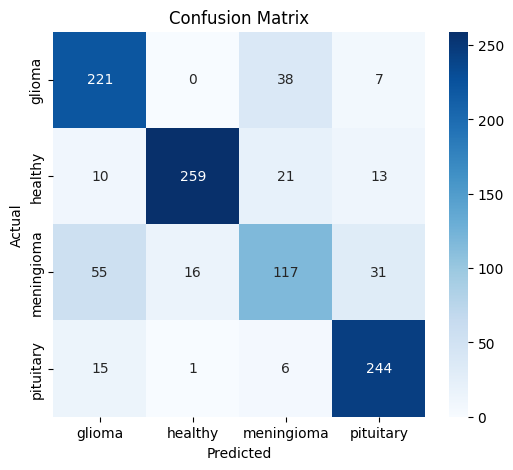
\includegraphics[width=1\linewidth]{scratchCM.png}
    \caption{Confusion Matrix: Scratch Model}
    \label{scratchCM}
\end{figure}
\begin{table}[h]
\centering
\caption{Classification Performance of the Scratch CNN Model}
\begin{tabular}{|l|c|c|c|}
\hline
\textbf{Class} & \textbf{Precision} & \textbf{Recall} & \textbf{F1-Score} \\
\hline
Glioma      & 0.73 & 0.83 & 0.78 \\
Healthy     & 0.94 & 0.85 & 0.89 \\
Meningioma  & 0.64 & 0.53 & 0.58 \\
Pituitary   & 0.83 & 0.92 & 0.87 \\
\hline
Weighted Avg & 0.80 & 0.80 & 0.79 \\
\hline
\end{tabular}
\label{tab:scratch_results}
\end{table}

Looking at Table \ref{tab:scratch_results} and Fig. \ref{scratchCM}, we observe that the CNN built from scratch achieved relatively strong precision, recall, and F1-score values across most classification categories. The model performed very well when classifying Pituitary and healthy MRI scans. It achieved an F1-score of 0.87 and 0.89 respectively. 

However, our model struggled when classifying MRI scans with meningioma tumors. The model only achieved an F1-score of 0.58. This indicates that the model is struggling to balance recall and precision. Taking a deeper look, we observe that the recall score for the meningioma tumor class is much lower than the precision score. This indicates that the model struggled to correctly identify the actual meningioma tumor images and a significant number of meningioma tumors were misclassified.

Looking at the glioma class, we observe that the precision score is much lower than the recall score. This indicates that of all the magnetic resonance images that were predicted to contain glioma tumors, only about 0.73 were actually glioma tumors. This shows that the model produced a large number of false positive predictions for this class. The pituitary class also has a lower precision score compared to the recall score. 

The healthy class achieved a precision score of 0.94, indicating that the model rarely classified tumor MRI scans as healthy. Of 276 MRI scans predicted to be healthy, only 17 instances contained tumors. Of the 17 misclassified scans, 16 belonged to the meningioma class. Once again, we observe that the model struggles with correctly identifying and classifying meningioma tumors. These results are very important in medical image classification because incorrectly predicting a tumor scan as healthy may delay diagnosis and treatment. Furthermore, it is far better to have a false positive compared to a false negative in medical diagnosis. We aim to improve the performance metrics with our model built using DenseNet-121.

\subsection{CNN with Transfer Learning}

The transfer learning CNN achieved a test accuracy of approximately 88\% with a test loss of 0.279. This is a much stronger model compared to the model built from scratch.
\begin{figure}[!htbp]
    \centering
    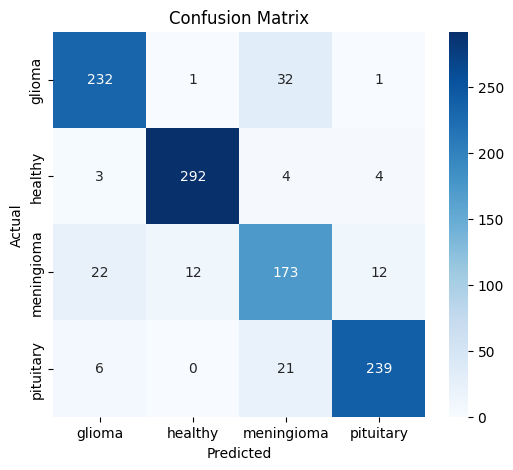
\includegraphics[width=1\linewidth]{transCM.png}
    \caption{Confusion Matrix: Transfer Learning}
    \label{transCM}
\end{figure}
\begin{table}[h]
\centering
\caption{Classification Performance of the DenseNet-121 Transfer Learning Model}
\begin{tabular}{|l|c|c|c|}
\hline
\textbf{Class} & \textbf{Precision} & \textbf{Recall} & \textbf{F1-Score} \\
\hline
Glioma      & 0.88 & 0.87 & 0.88 \\
Healthy     & 0.96 & 0.96 & 0.96 \\
Meningioma  & 0.75 & 0.79 & 0.77 \\
Pituitary   & 0.93 & 0.90 & 0.92 \\
\hline
Weighted Avg & 0.89 & 0.89 & 0.89 \\
\hline
\end{tabular}
\label{tab:transfer_results}
\end{table}

Looking at Table \ref{tab:transfer_results} and Fig. \ref{transCM}, we observe that the CNN built with transfer learning achieved a much stronger precision, recall, and F1-score values compared to the model built from scratch. The model performed very well when classifying Pituitary and healthy MRI scans. It achieved an F1-score of 0.92 and 0.96 respectively. 

Once again, we observe that our model struggled when classifying MRI scans with meningioma tumors. However, the F1-score changed from 0.58 to 0.77 when compared to the scratch model. This indicates that transfer learning with DenseNet-121 significantly improved the model’s ability to classify meningioma tumors. Taking a deeper look, we observe that the precision and recall scores for the meningioma tumor class has jumped from 0.64 and 0.53 to 0.75 and 0.79 respectively. 

Looking at the glioma class, we also observe improvements in precision and recall scores. The glioma class previously achieved precision and recall scores of 0.73 and 0.83, but improved to 0.88 and 0.87 respectively. In addition, the pituitary class precision improved from 0.83 to 0.93. However, the recall score slightly dropped from 0.92 to 0.90. Overall, this is an improvement since the F1-score improved significantly.

The healthy class achieved precision, recall, and F1-score values of 0.96, indicating that the model rarely classified tumor MRI scans as healthy. Of 305 MRI scans predicted to be healthy, only 13 instances contained tumors. Of the 13 misclassified scans, 12 belonged to the meningioma class. Once again, we observe that the model struggles with correctly identifying and classifying meningioma tumors. However, this is a significant improvement compared to the model built from scratch. This demonstrates the effectiveness of transfer learning for medical image classification tasks.

\section{Explainable AI}

\subsection{Grad-CAM}

To improve interpretability and better understand the decision-making process of the CNN models, Gradient-weighted Class Activation Mapping (Grad-CAM) was utilized. Grad-CAM is an Explainable Artificial Intelligence (XAI) technique that visually highlights the regions in an image that are most important to influencing the model's prediction.

Grad-CAM first performs a forward pass through the CNN to get the feature maps and raw outputs from the final convolutional layer. These are taken from the final layer as these features have the most semantically rich features. The feature maps are denoted as $A^k$, where $k$ refers to one specific feature map within the convolutional layer. Next, the target class is selected. This is typically the class with the highest prediction score. $y^c$ represents the score for class $c$, which is the raw output value for class $c$. After this, the gradient of the target class score is computed with respect to the feature maps. The partial derivative specifically tells us how important each feature map is for the target class. If a tiny change in a feature map causes a large change in the tumor prediction, then that feature map is important. The partial derivative is written as,
\[
\frac{\partial y^c}{\partial A^k}
\]

For every filter, $k$, the gradients are then globally averaged to determine how important each feature map is for the selected class. The following equation gives us the overall importance weight for the entire feature map,

\[
\alpha_k^c = \frac{1}{Z} \sum_i \sum_j \frac{\partial y^c}{\partial A_{ij}^k}
\]

where $y^c$ is the score for class $c$, $A^k$ represents the feature map for filter $k$, $i$ and $j$ represent the width and height respectively, and Z represents the total number of pixels in the feature map.

Each feature map, $A^k$, is then multiplied by its corresponding importance weight, $\alpha_k^c$ and is summed over all filters. The ReLU function is then applied to keep only the values that positively impact the target class. This results in the final equation,
\[
L_{\text{Grad-CAM}}^c = \text{ReLU}\left(\sum_k \alpha_k^c A^k\right)
\]
Finally, the heatmap is resized to fit the input size and is overlayed onto the original MRI scan. This allows visualization of the areas the CNN considered the most important during classification. By visualizing these important regions, Grad-CAM improves model transparency and provides insight into the most important features of the image. It displays how the model made its final prediction \cite{gradcamtutorial}.

\subsection{Grad-CAM Visualization}
\begin{figure}[!htbp]
\centering

\begin{minipage}[b]{0.24\textwidth}
    \centering
    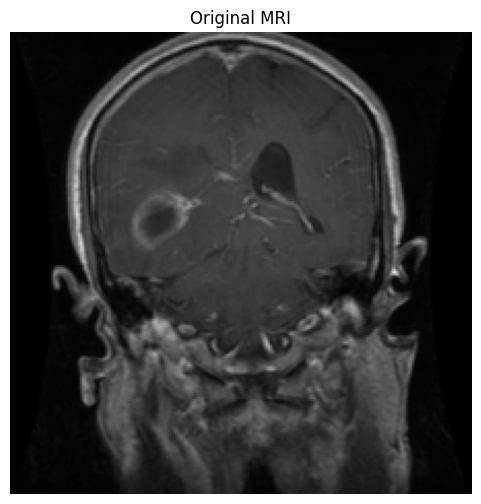
\includegraphics[width=\textwidth]{xai2.png}
\end{minipage}
\hspace{0.01\textwidth}
\begin{minipage}[b]{0.24\textwidth}
    \centering
    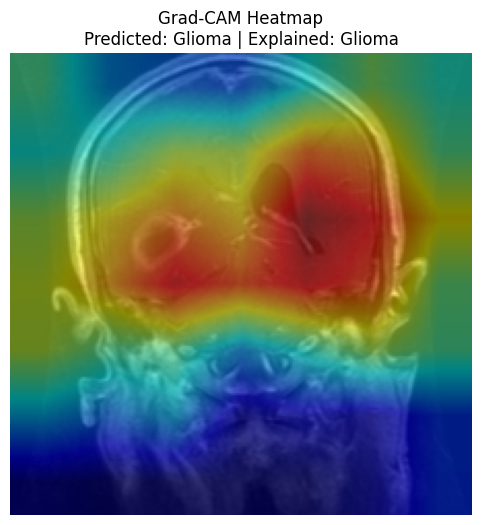
\includegraphics[width=\textwidth]{xai2.2.png}
\end{minipage}

\caption{Original Glioma MRI scan and corresponding Grad-CAM heatmap visualization.}
\label{fig:xai_combined}

\end{figure}

The Grad-CAM visualization in Fig. \ref{fig:xai_combined} demonstrates that the CNN focused strongly on the tumor region when predicting the glioma class. The heatmap concentrates around the abnormalities within the brain. Although the heatmap includes some outer edges, this figure still illustrates the abilities of the deep learning model to not only classify brain tumors, but to also highlight the important regions of the MRI. 

\begin{figure}[!htbp]
\centering

\begin{minipage}[b]{0.24\textwidth}
    \centering
    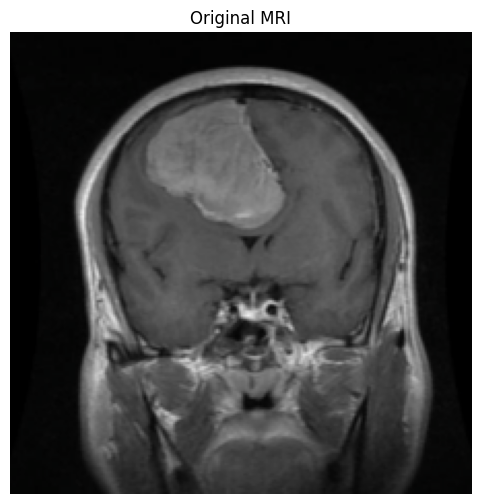
\includegraphics[width=\textwidth]{xai3.png}
\end{minipage}
\hspace{0.01\textwidth}
\begin{minipage}[b]{0.24\textwidth}
    \centering
    
\includegraphics[width=\textwidth]{xai3.1.png}
\end{minipage}

\caption{Original Meningioma MRI scan and corresponding Grad-CAM heatmap visualization.}
\label{fig:xai_combined2}

\end{figure}

\begin{figure}[!htbp]
\centering

\begin{minipage}[b]{0.24\textwidth}
    \centering
    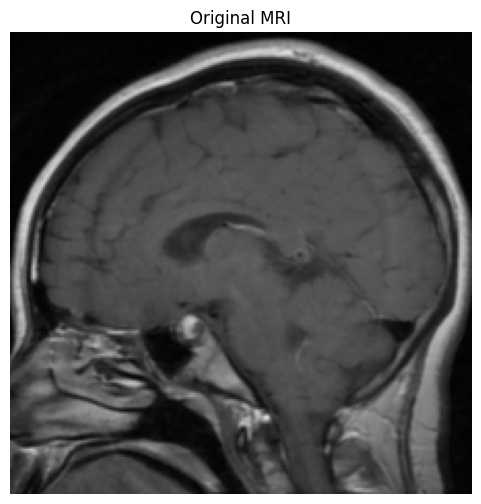
\includegraphics[width=\textwidth]{xai4.png}
\end{minipage}
\hspace{0.01\textwidth}
\begin{minipage}[b]{0.24\textwidth}
    \centering
    
\includegraphics[width=\textwidth]{xai4.1.png}
\end{minipage}

\caption{Original Pituitary MRI scan and corresponding Grad-CAM heatmap visualization.}
\label{fig:xai_combined3}

\end{figure}

In Fig. \ref{fig:xai_combined2}, Grad-CAM highlights the tumor region that contributes to the model's prediction. This particular example showcases the meningioma tumor that our model tends to struggle with. However, this is a very good example that proves the model is able to learn medically relevant image features during classification.

In Fig. \ref{fig:xai_combined3}, the Grad-CAM methods highlights regions near the pituitary gland when predicting the pituitary tumor class. Once again, we see that the method is effective in highlighting the important regions of the MRI. However, the heatmap is never perfect and also highlights areas around the pituitary gland. Overall, we are able to observe the effectiveness of the XAI techniques.


\section{Conclusion}
In this study, we developed two deep learning models for brain tumor classification. A baseline CNN was built from scratch to establish a baseline for our task. We then fine-tuned a CNN by incorporating transfer learning using the DenseNet-121 architecture. The transfer learning model achieved significant results when classifying brain tumor among MRI scans. Additionally, we incorporated Grad-CAM XAI techniques to display a heatmap over the MRI image to highlight relevant features within the image. Overall, this project shows the capabilities of deep learning models and XAI techniques. The work also supports medical professionals in identifying and classifying brain tumors.

\section{Future Work}
Future work for this research includes exploring other XAI techniques. More specifically, we want to explore other techniques that improve localization of the tumors. These methods include Score-CAM, LayerCAM, and Grad-CAM++. One of the biggest limitations of this research was the dataset. Medical images are often private, making it difficult to explore more research.
\begin{thebibliography}{00}

\bibitem{bhandari}
Bhandari, A., Koppen, J., \& Agzarian, M. (2021). \emph{Convolutional Neural Networks for Brain Tumor Segmentation: A Review}. 
Frontiers in Computational Neuroscience, 15. 
Available: \url{https://pmc.ncbi.nlm.nih.gov/articles/PMC8300985/}

\bibitem{bhanothu2020}
Bhanothu, Y., Kamalakannan, A., \& Rajamanickam, G. (2020). \emph{Detection and Classification of Brain Tumor in MRI Images using Deep Convolutional Network}. 
2020 6th International Conference on Advanced Computing and Communication Systems (ICACCS). 
Available: \url{https://ieeexplore.ieee.org/document/9074375}

\bibitem{gayanga2019}
Gayanga, T. D. L., Pathirana, G. P. S. N., \& Sandanayake, T. C. (2019). \emph{Detecting and Capturing the Intensity of a Brain Tumor using MRI Images}. 
2019 4th International Conference on Information Technology Research (ICITR). 
Available: \url{https://ieeexplore.ieee.org/document/9407795}

\bibitem{ncneurospine}
Neurosciences \& Spine Center. (2026). \emph{The Importance of Early Detection in Brain Tumors}. 
Available: \url{https://www.ncneurospine.com/the-importance-of-early-detection-in-brain-tumors/}


\bibitem{gradcamtutorial}
XAI Tutorials. (2024). \emph{Grad-CAM}. 
Available: \url{https://xai-tutorials.readthedocs.io/en/latest/_model_specific_xai/Grad-CAM.html}

\bibitem{ibmcnn}
IBM. (2024). \emph{What are Convolutional Neural Networks?} 
Available: \url{https://www.ibm.com/think/topics/convolutional-neural-networks}

\end{thebibliography}

\end{document}
